% MATLAB source: paper/plot_existing_manuscript_figures.m
\begin{figure}[tbp]
  \centering
  \begin{subfigure}[t]{0.94\linewidth}
    \centering
    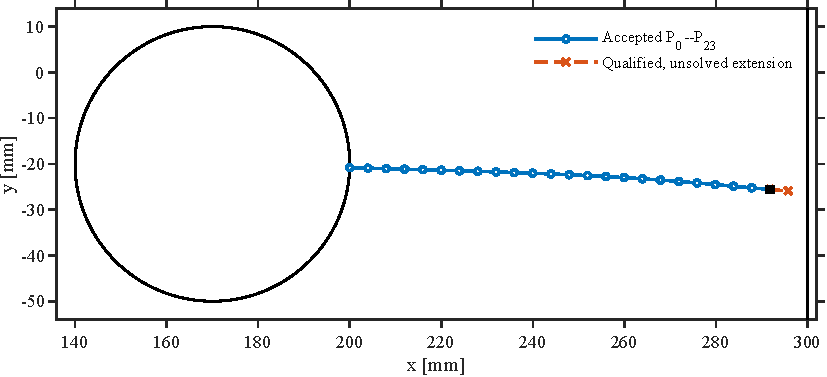
\includegraphics[width=\linewidth]{figures/trajectory/overview.pdf}
    \caption{Hole and accepted trajectory through $P_{23}$, with the
    qualified but physically unsolved $P_{23}$--$P_{24}$ extension.}
    \label{fig:trajectory-overview}
  \end{subfigure}

  \medskip

  \begin{subfigure}[t]{0.94\linewidth}
    \centering
    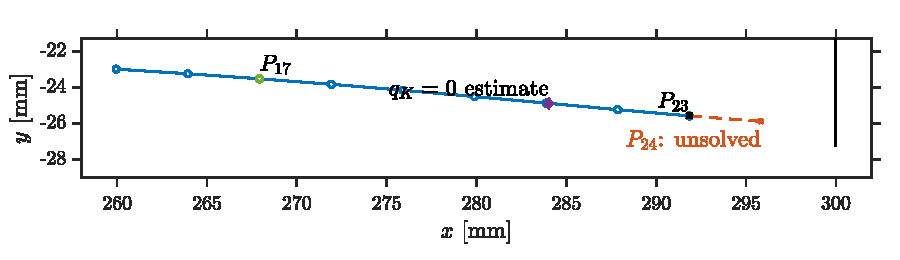
\includegraphics[width=\linewidth]{figures/trajectory/late_detail.pdf}
    \caption{Late-path detail with equal spatial scales. The markers identify
    $P_{17}$, the linearly interpolated $K_{II}/K_I=0$ location, $P_{23}$,
    and the qualified unsolved point $P_{24}$.}
    \label{fig:trajectory-late}
  \end{subfigure}

  \caption{Hole-initiated trajectory and late detail. Both spatial panels
  use equal $x$ and $y$ scales within the panel. The circle gives geometric
  context; the numerical hole is polygonally discretized. Solid segments are
  accepted geometry through $P_{23}$. The dashed extension is qualified
  geometry only and has no accepted physical SIFs. The diamond is a linear
  interpolation marker, not a solved tip.}
  \label{fig:trajectory}
\end{figure}
